% 斯托克斯定理
% 曲面|闭合曲线|环流量

\begin{issues}
\issueTODO
\end{issues}

\pentry{旋度\upref{Curl}}

\begin{figure}[ht]
\centering
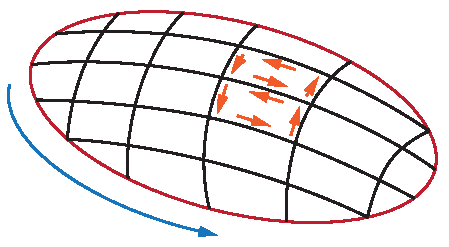
\includegraphics[width=6cm]{./figures/Stokes_1.pdf}
\caption{斯托克斯定理} \label{Stokes_fig1}
\end{figure}

如\autoref{Stokes_fig1}, 我们选取一块曲面, 并规定一个正方向. 使用右手定则\upref{RHRul}, 我们也可以定义曲面边界的正方向. 空间中存在连续光滑的矢量场 $\bvec F(\bvec r)$, 则\textbf{斯托克斯定理}可以将矢量场在曲面边界上的环流量和矢量场的旋度在曲面上通量等同起来
\begin{equation}
\oint \bvec F(\bvec r) \vdot \dd{\bvec r} = \int \curl \bvec F(\bvec r) \vdot \dd{\bvec s}
\end{equation}


要证明这个定理, 我们将曲面划分为许多小面元 $\Delta \bvec s_i$, 其正方向与曲面一致, 边界的正方向同样由右手定则定义. 这样, 矢量场在曲面上的通量就等于在每个小面元上的通量之和. 当面元的面积趋于零时, 我们可以认为场的旋度在面元上是常矢量 $\bvec F(\bvec r_i)$, $\bvec r_i$ 为 $\Delta \bvec s_i$ 上任意一点. 由\autoref{Curl_eq3} 可知面元的环流量为 $\curl\bvec F(\bvec r_i) \vdot \Delta \bvec s_i$(可类比\autoref{Diff_eq2}~\upref{Diff}), 所以根据积分的思想, 所有面元的环流量之和为
\begin{equation}
\lim_{\Delta s_i \to 0}\sum_i \curl\bvec F(\bvec r_i) \vdot \Delta \bvec s_i = \int \curl\bvec F(\bvec r) \vdot \dd{\bvec s}
\end{equation}
最后, 如何证明所有面元的环流量之和等于曲面边界的环流量呢? 类比散度定理(\autoref{Divgnc_eq13}~\upref{Divgnc})的证明, 考虑任意两块相邻的小面元, 矢量场在它们共同边界的线积分对一个面元的环流量贡献为正, 而对另一个面元的环流量贡献大小相同但符号为负, 所以在上式的求和中相加为零. 所以, 求和中唯一没有被抵消的环流量来自于曲面边界处的面元, 这些面元的边界与曲面边界重合且正方向一致, 对求和的贡献恰好等于曲面边界的环流量. 证毕.

\addTODO{例题}
